\subsection{Calibration}

First we have to calibrate the system. We only measure the number of entries in different channels, but we know at which energies the spectrum of ${}^{22}\mathrm{Na}$, $^{60}\mathrm{Co}$ and $^{137}\mathrm{Cs}$ have peaks due to radiation. With these values we can make a linear regression and map the channels onto energies. \\
Fig.2.1 shows the entries in each channel for ${}^{22}\mathrm{Na}$ as an example. We fitted the peak with a gaussian function to get a better estimated value. \\
In Fig.2.2 you can see the channels of each peak and the corresponding energies. Fig.2.3 finally shows the linear regression with the following parameters:
$$\mathrm{y-intercept} = (-3.02810 \pm 1.48205) \cdot 10^{2} \ keV$$
$$\mathrm{slope} =  (3.64232 \pm 0.513385) \ keV$$

\begin{figure}[h]
\centering
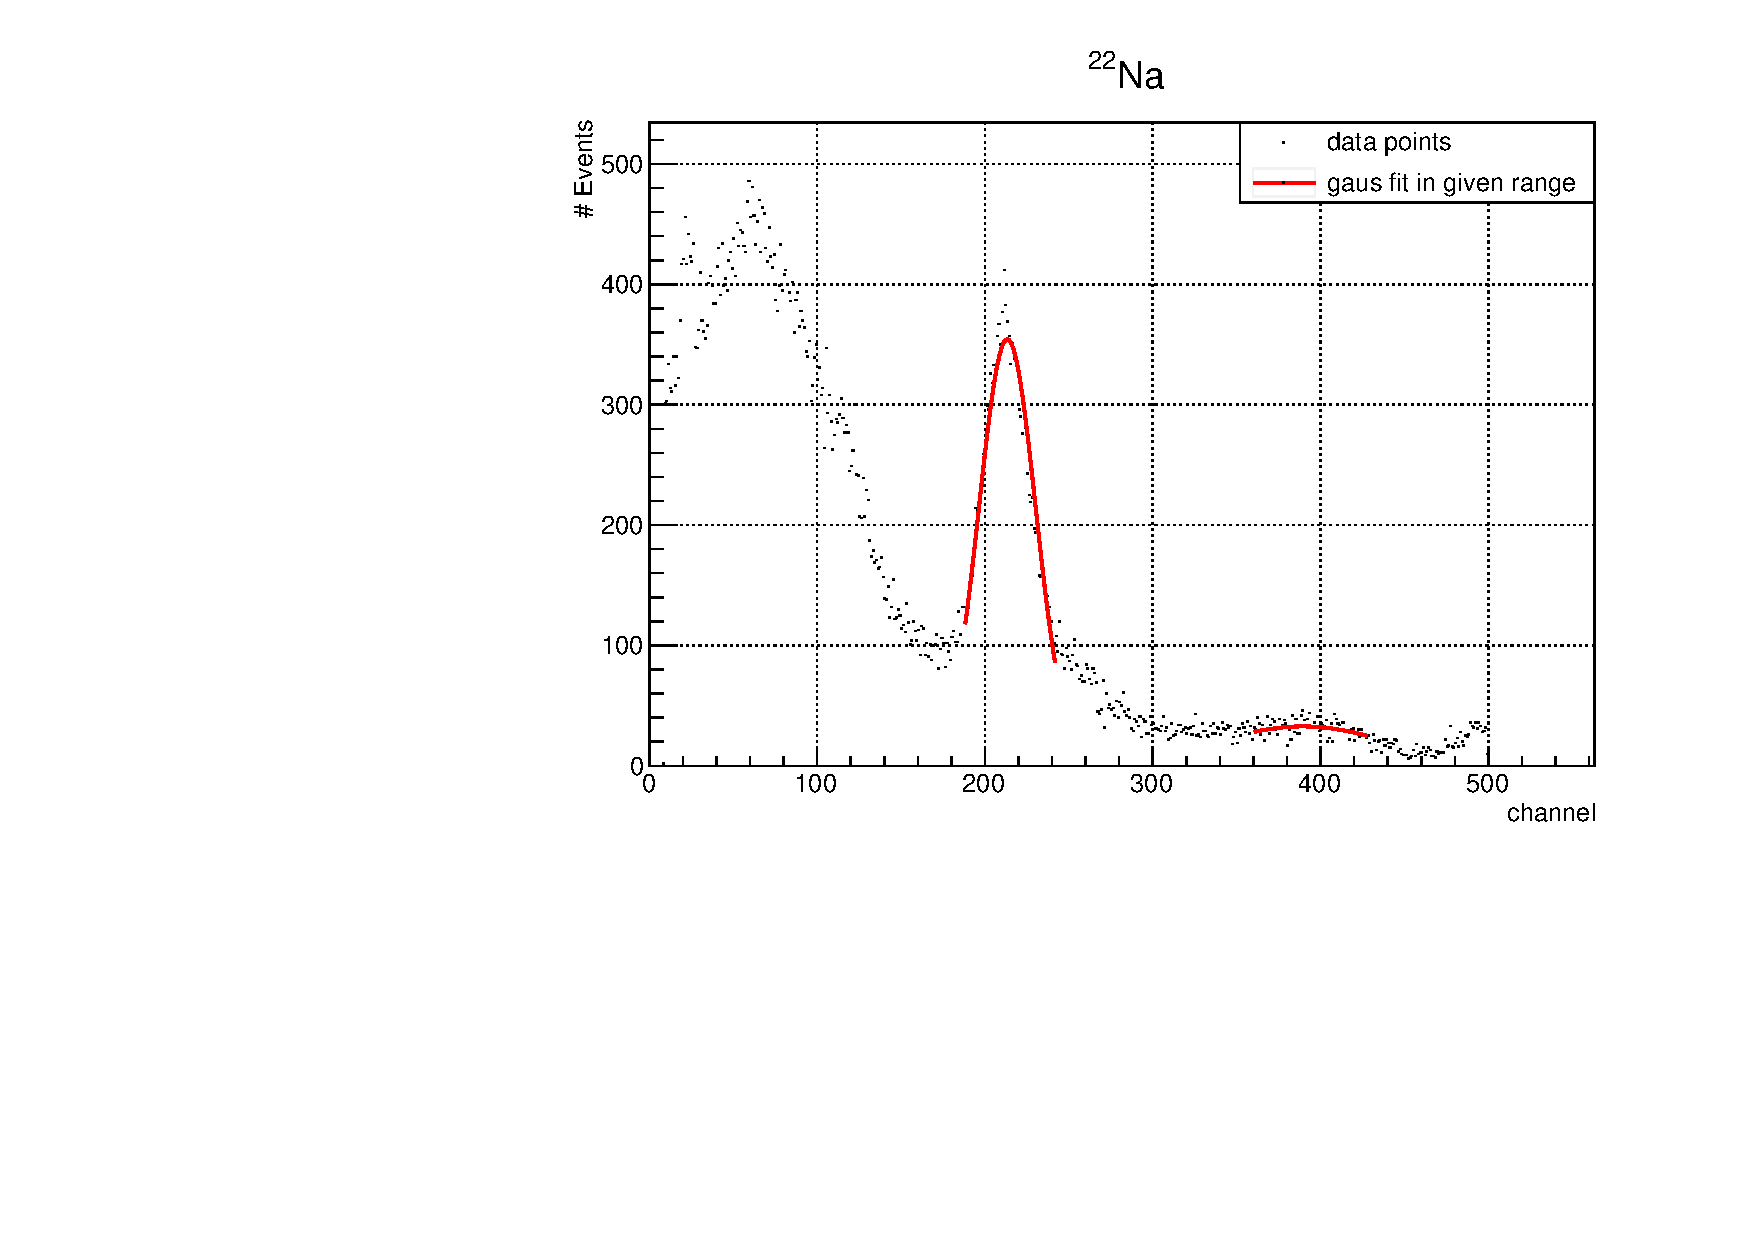
\includegraphics[scale=0.5]{./../plots/calibration/NA_22_fit.pdf}
\caption{Measured channels for ${}^{22}\mathrm{Na}$. At estimated ranges we fitted gaussian distributions to get better estimates of the peaks.}
\end{figure}

\newpage

\begin{figure}[h]
\centering
\caption{Measured channels and corresponding energies. Data for a linear fit.}
\vspace{0.2cm}
\begin{tabular}{lccc}
& mean & sigma & energy in keV \\
\hline
\hline
\vspace{0.1cm}
${}^{22}\mathrm{Na}$ & 213.33 & 16.88 & 511.0 \\
${}^{22}\mathrm{Na}$ & 389.31 & 52.35 & 1274.6 \\
$^{60}\mathrm{Co}$ & 362.87 & 68.07 & 1173.2 \\
$^{60}\mathrm{Co}$ & 463.79 & 32.98 & 1332.6 \\
$^{137}\mathrm{Cs}$ & 278.01 & 16.78 & 661.7 \\
\end{tabular}
\end{figure}

\begin{figure}[h]
\centering
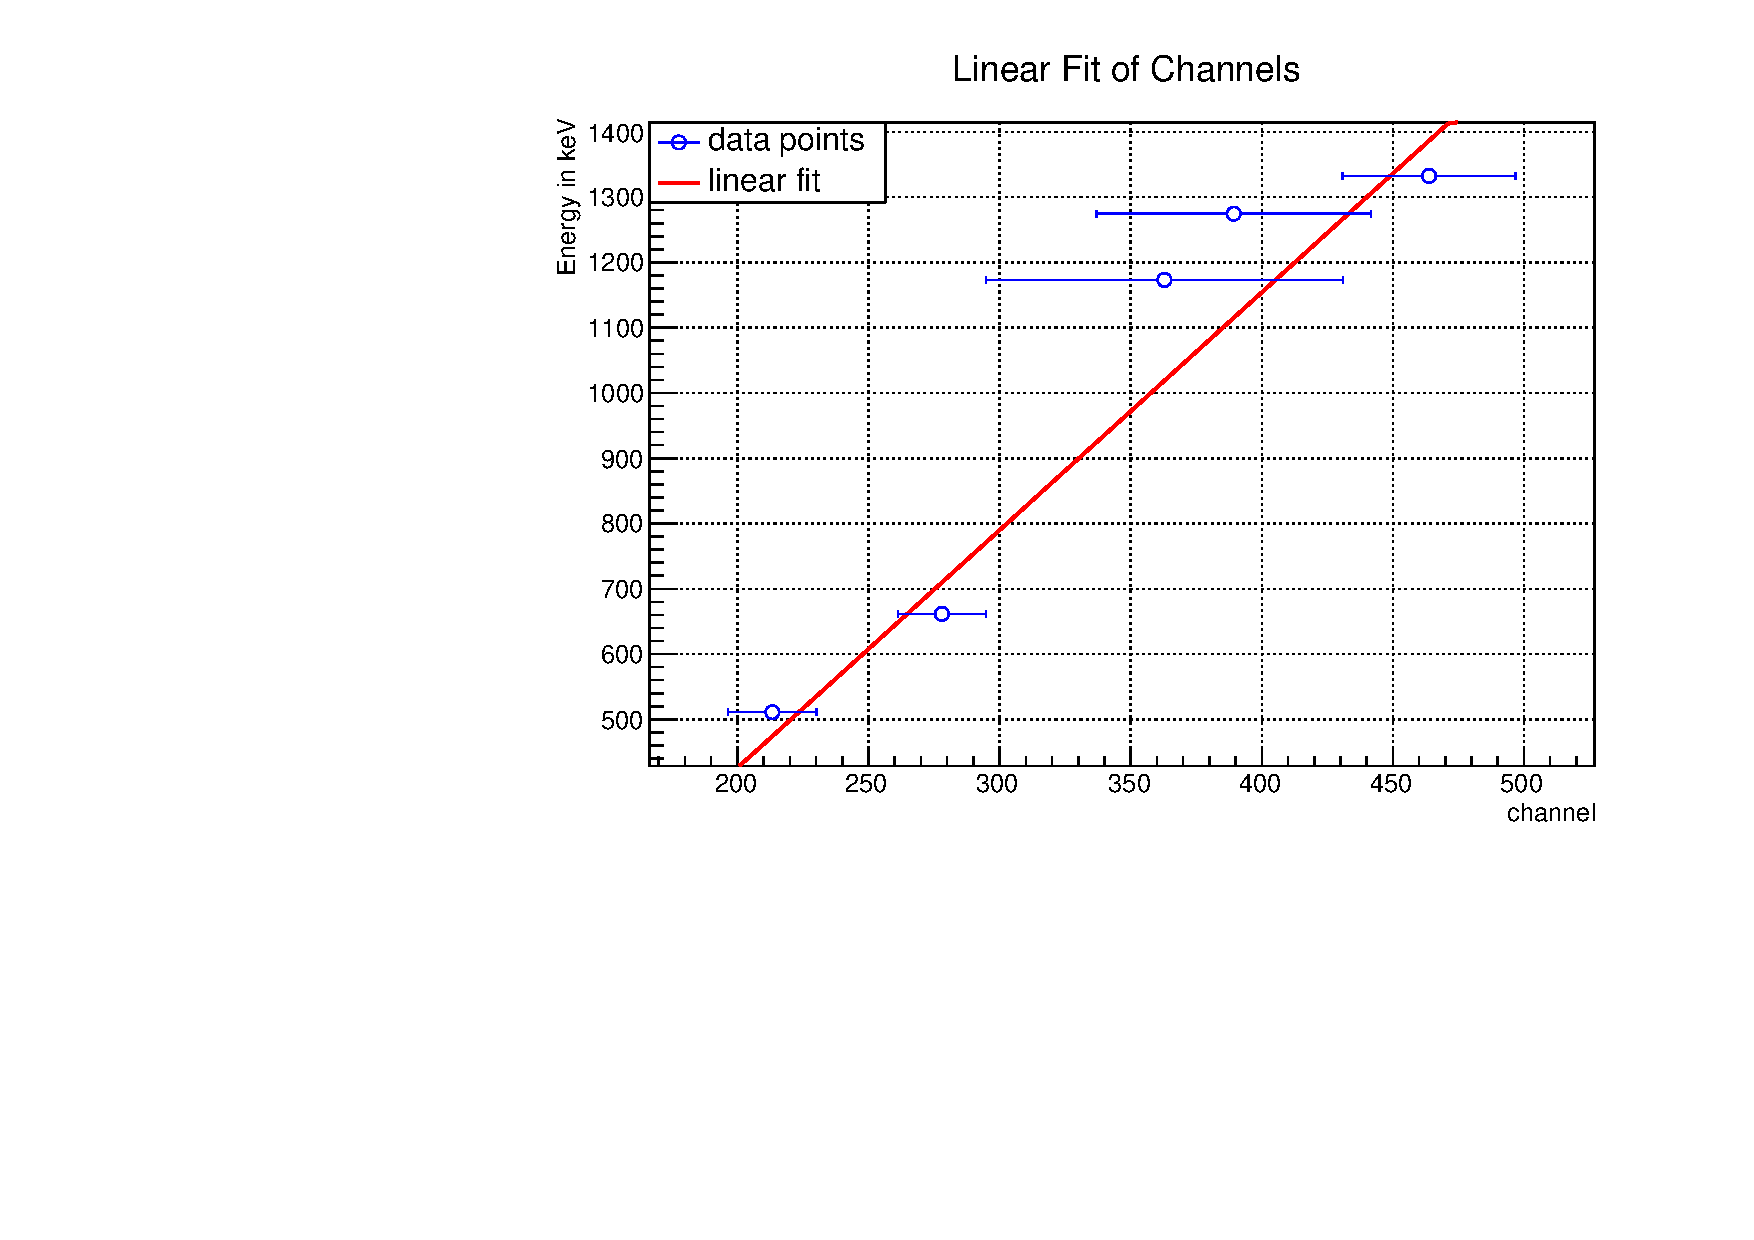
\includegraphics[scale=0.5]{./../plots/calibration/lin_fit.pdf}
\caption{Linear fit of channels and corresponding energies. The slope and intersection make it possible so that we can map the channels on the energies.}
\end{figure}


\newpage

\subsection{Differential Cross Section}

Next we measure the diffential cross section with respect to the solid angle $\Omega$. We assume that it has a rotation symmetry, i.e. it is independend of the azimuth $\phi$.\\
We change the angle in $10 ^{\circ}$ steps ranging from $20 ^{\circ}$ to $100 ^{\circ}$ and measure the background without target and the events with target. The sum of the difference is the total number scattered $R$. \\
To calculate the cross section we use the formular given in corresponding part of the preparation. The values used are in the appendix. To mention is the decay of the source, so we had to correct it by a factor $2^{-t/t_{1/2}}$ with $t_{1/2} = 30a$ and $t = 2016 - 1971 = 45a$. We also multiplied this value by the time we measured the events $t_{meassurement} = 300s$\\
Fig.2.4 shows the polar angle $\Theta$ and the measured cross section with its errors.

\vspace{5cm}

\begin{figure}[h]
\centering
\caption{Angles $\Theta$ and the measured differential cross section in $cm^{-2}$.}
\vspace{0.2cm}
\begin{tabular}{lcc}
$\Theta$ in ${}^{\circ}$ & $\frac{\mathrm{d}\sigma}{\mathrm{d}\Omega}$ in $cm^{-2}$ & error of the cross section  \\
\hline
\hline
%\vspace*{0.1cm}
20     &  0.684 & 0.041 \\
30     &  0.558 & 0.033 \\
40     &  0.442 & 0.026 \\
50     &  0.348 & 0.021 \\
60     &  0.282 & 0.017 \\
70     &  0.240 & 0.014 \\
80     &  0.212 & 0.013 \\
90     &  0.204 & 0.012 \\
100    &  0.200 & 0.012 \\
\end{tabular}
\end{figure}

\newpage

\subsection{Energy Shift and Invariant Mass of Electrons}

The energy of a fixed angle is determined by a gaussian fit, an example is shown in Fig.2.5 for $\Theta = 50^{\circ}$. The procedure is the same as in the calibration subsection above. Using the measured linear fit from above we can acquire the energies from the channels.\\
As described in the preparation we plot the inverse energy $\frac{1}{E}$ over $1 - \cos(\Theta)$. The inverse of the slope gives the invariant mass of the electron in $keV$. The resulting plot is given in Fig.2.6 with following parameters for the fit:
$$\mathrm{y-intercept} = (1.20237 \pm 0.553517) \cdot 10^{-4} \ keV$$
$$\mathrm{slope} =  (4.55878 \pm 3.02294) \cdot 10^{-3} \ keV$$
As a result we can calculate the electron mass to be:
$$(219.357 \pm 145.456) \ keV$$

The uncertainty for $\frac{1}{E}$ is calculated by 
$$\sigma _{energy}^{2} = (\frac{1}{slope})^{2} \cdot (\sigma _{channel} ^{2} + \sigma _{intercept} ^{2} + (channel - intercept)^{2} \cdot (\frac{\sigma_{slope}}{slope})^{2}) $$
Since $\sigma _{intercept}$ is a big number originating from the calibration and it is present even for small values of ${E}$, it dominates the uncertainty in these regime. The result is a big absolute uncertainty for big values of the inverse energy $\frac{1}{E}$, which is the reason for the graph above.

\begin{figure}[h]
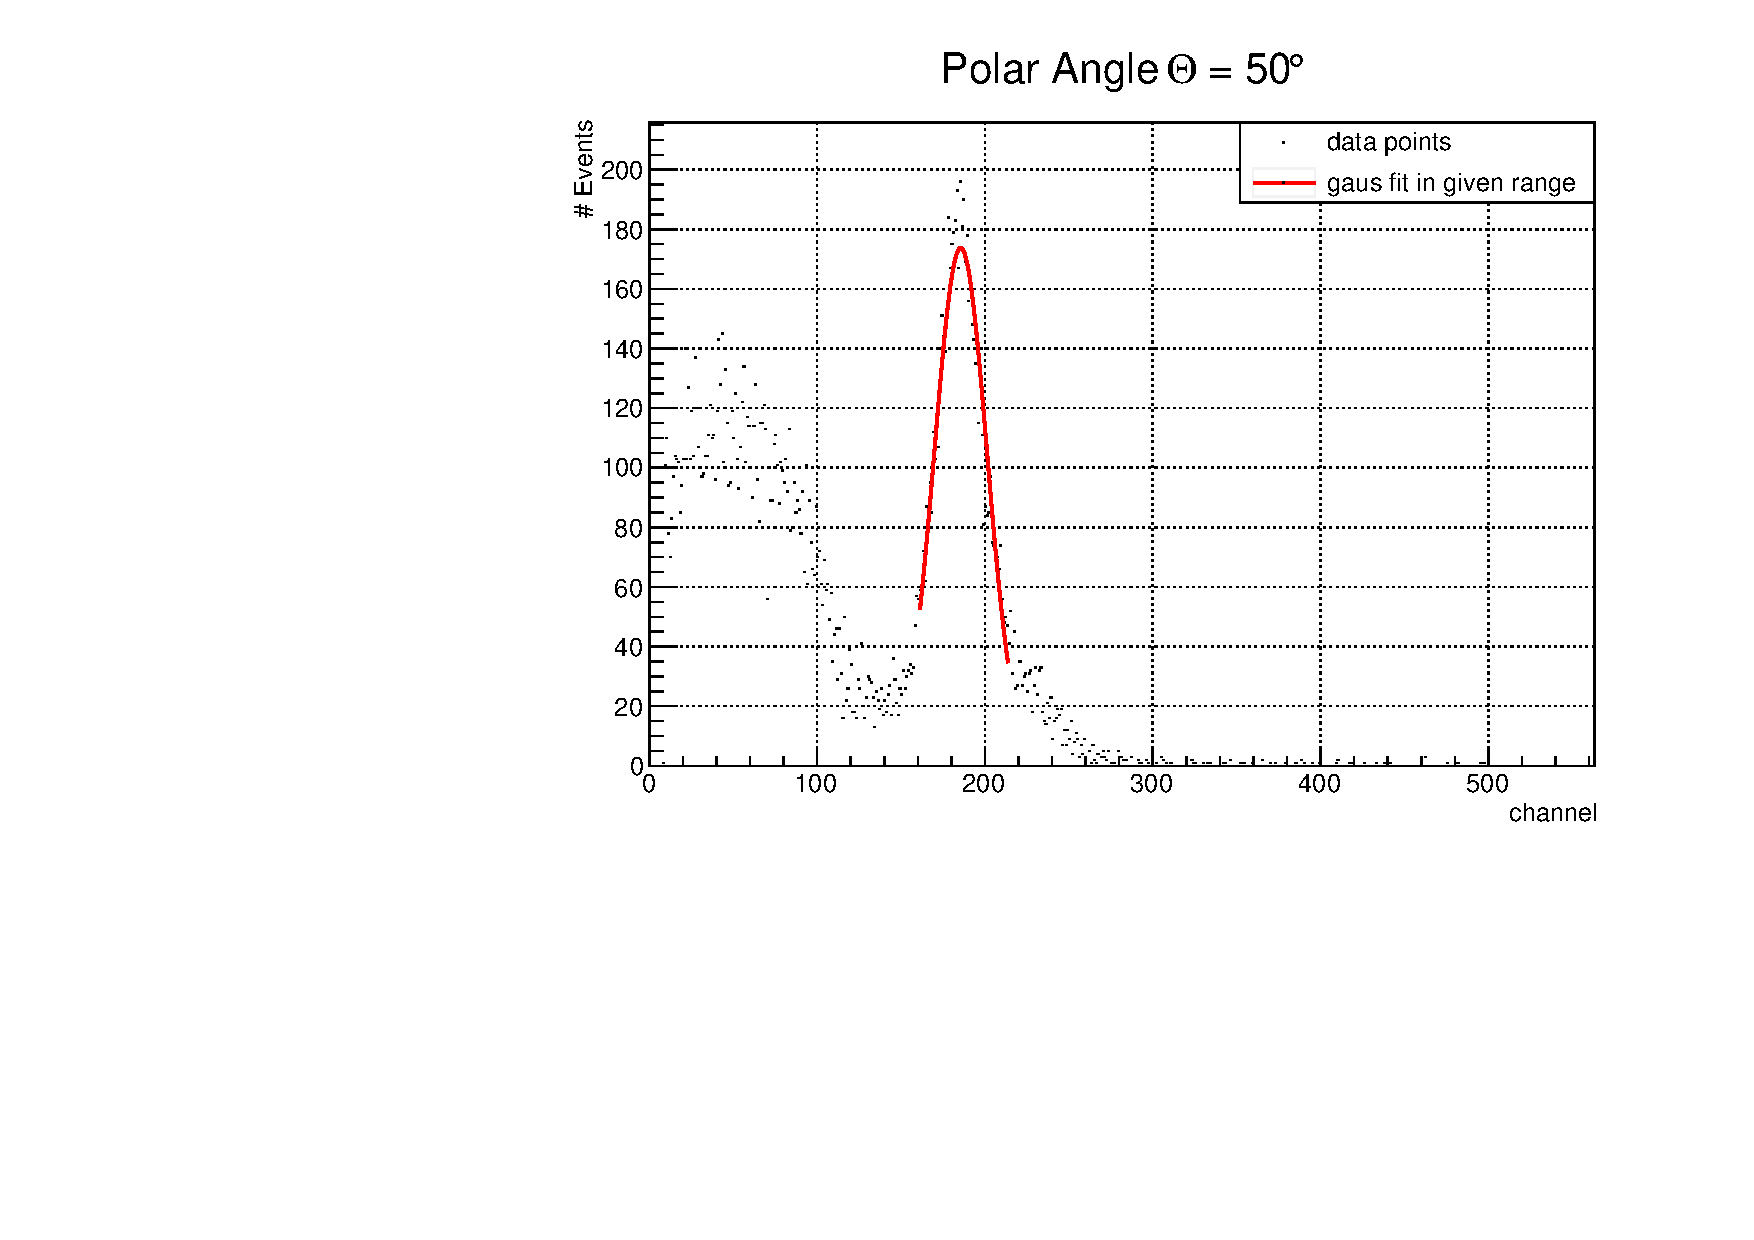
\includegraphics[scale=0.5]{./../plots/50_deg.pdf}
\caption{Fit to determine the energy at a fixed angle of $\Theta = 50^{\circ}$.}
\end{figure}

\newpage

\begin{figure}
\centering
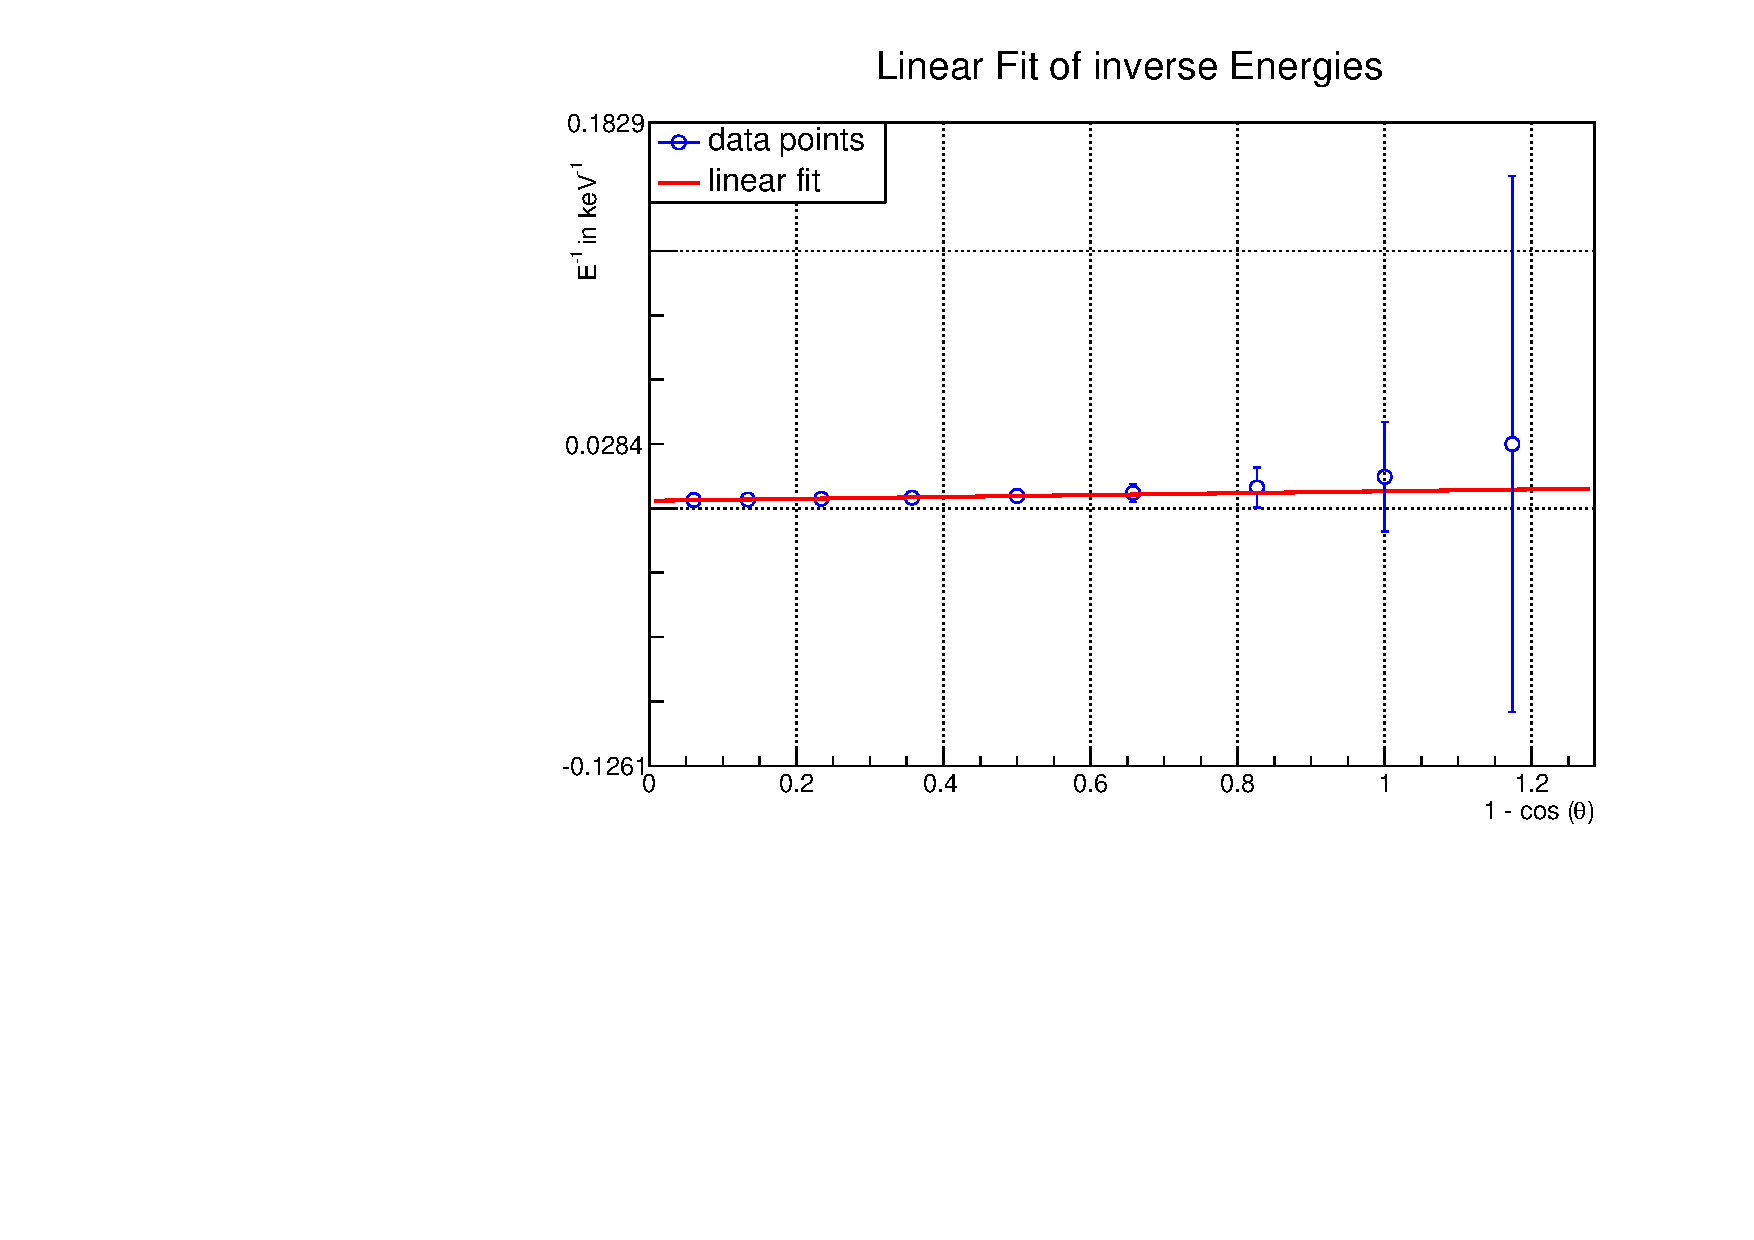
\includegraphics[scale=0.5]{./../plots/inv_el_mass.pdf}
\caption{Fit to determine the invariant mass of electrons. The uncertainty is big for high values of $\frac{1}{E}$ due to the big uncertainty of the y-intercept in the calibration fit.}
\end{figure}


\subsection{Cross Section for Different Materials}

As described in the preparation the following formular should be true given that the binding energy is much smaller than the energy of the photons:
$$(\frac{\mathrm{d}\sigma}{\mathrm{d}\Omega})_e = const. \cdot R \frac{A}{\rho Z} $$
We measured the total number of events for a fixed angle $\Theta = 20 ^{\circ}$ for different targets and subtracted the background $R = R_{target} - R_{background}$. The materials are aluminium, copper, iron and lead. Each target has the same size and shape. \\
To check the formular above we plot $\frac{R \cdot A}{\rho Z}$ over $Z$. This should be a horizontal line. Here $A$ is the atomic mass, $\rho$ is the density of the material and $Z$ is the atomic number. The used values are given in Fig.2.7.\\
\\
The resulting graph is shown in Fig.2.8. All data points except the one for lead are on a horizontal line. The reason is that the binding energy of lead is higher than for the others. Therefore the equation above doesn't hold true anymore because the electrons can't be simplified to be free anymore. It seems that with increasing atomic number, the error gets bigger. 

\newpage

\begin{figure}[h]
\centering
\caption{Values used for the different materials in the equation above.}
\vspace{0.2cm}
\begin{tabular}{lcccc}
 & aluminium  & copper & iron & lead  \\
\hline
\hline
$\rho$ in $\frac{g}{cm^{3}}$ & 2.70 & 8.92 & 7.87 & 11.34 \\
$A$ in $u$ & 26.98 & 63.55 & 55.85 & 207.2 \\
$Z$ & 13 & 29 & 26 & 82 \\
$R$ & 19619 & 58964 & 55038 & 50573 \\
$\sigma (R)$ & 1265.54 & 3688.28 & 3455.20 & 3477.25 \\
\end{tabular}
\end{figure}


\begin{figure}[h]
\centering
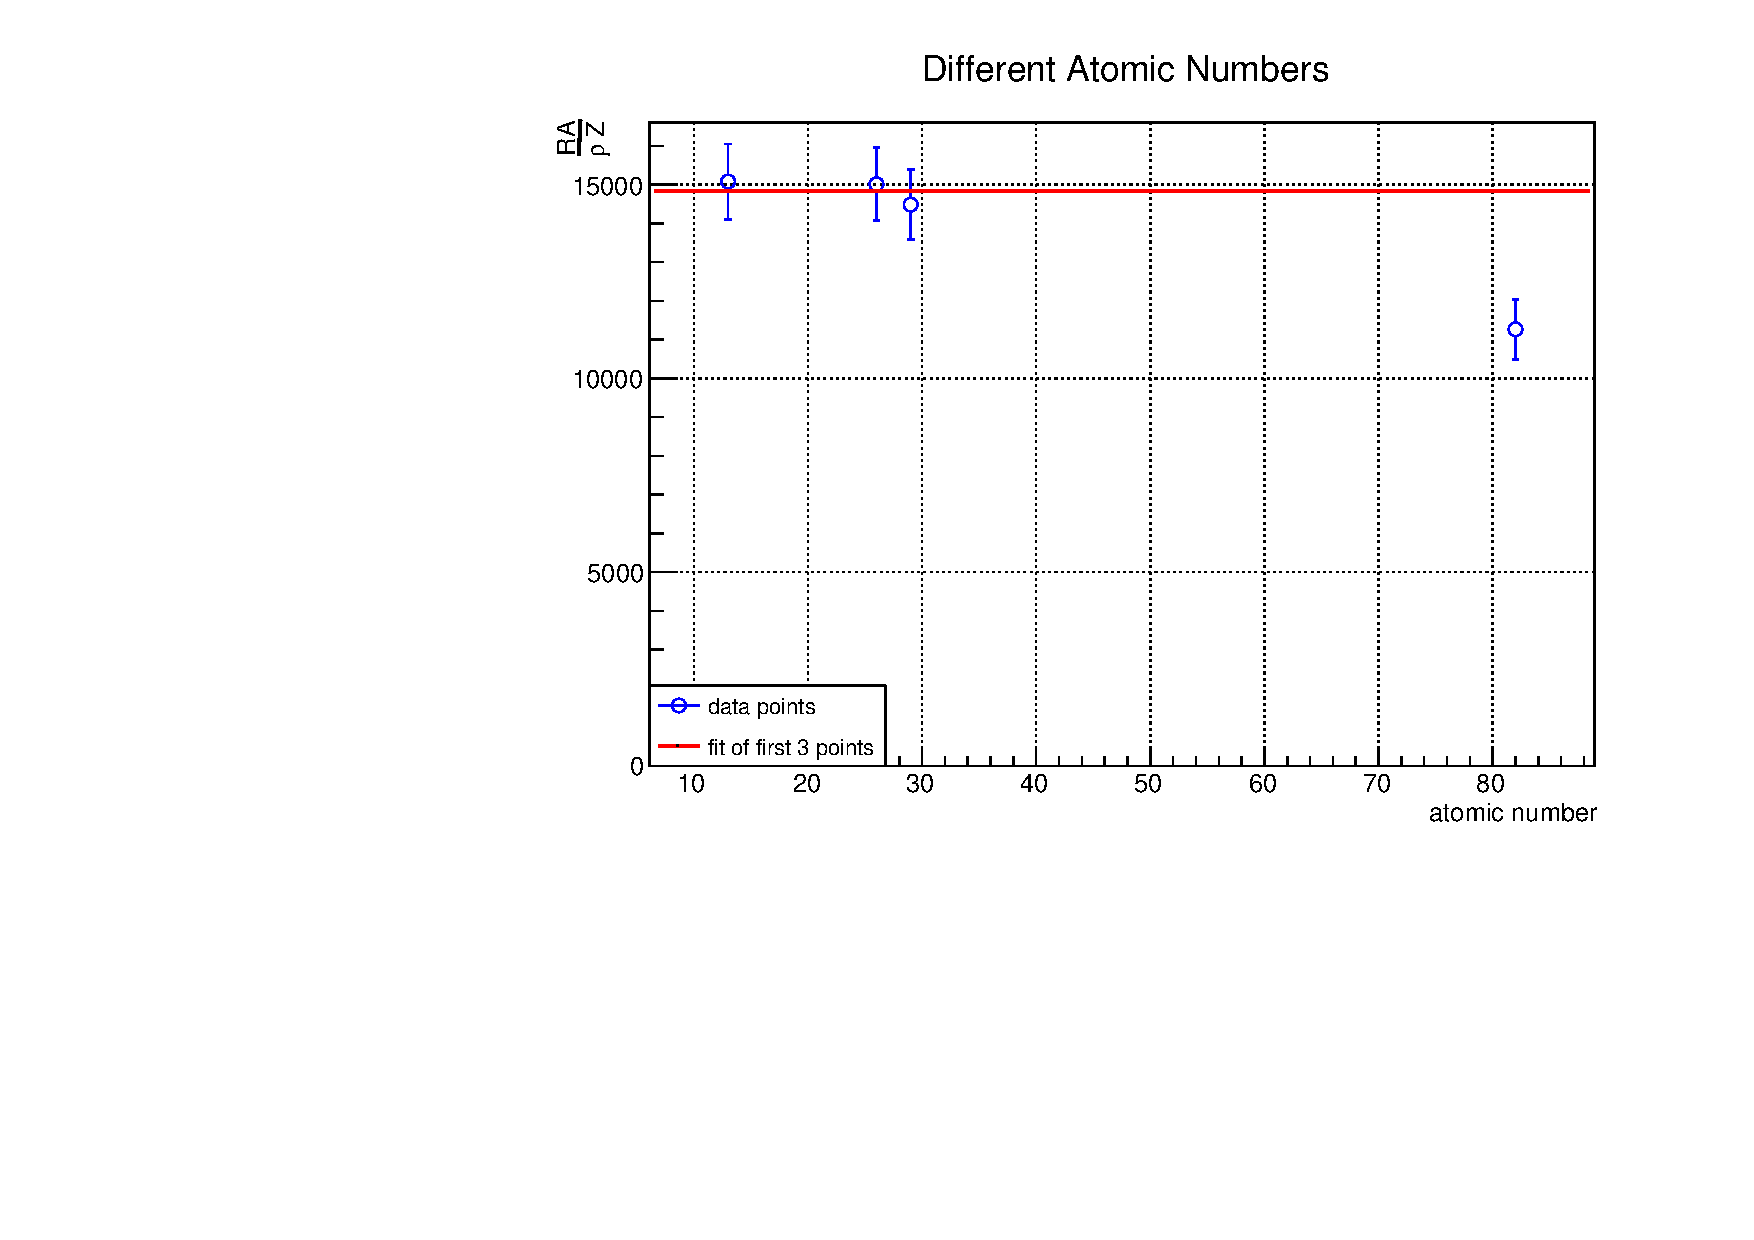
\includegraphics[scale=0.5]{./../plots/part_c.pdf}
\caption{Plot of the quantity mentioned in the text over the atomic number Z with a fit of the first three data points. Lead doesn't align with the other materials. The reason is the binding energy of the electrons.}
\end{figure}
